\documentclass[aspectratio=169]{beamer}
\usetheme{default}
\usecolortheme{rose}
\usepackage{graphicx}
\setbeamertemplate{caption}[numbered]
\graphicspath{{../figures/}}
\usepackage{subcaption}



\title{RTM Imaging}
\author{Clay Wood}
\date{06 May 2020}



\begin{document}
	
	
\begin{frame}[plain]
    \maketitle
\end{frame}


\begin{frame}{Reverse Time Migration Background}
	\begin{itemize}
		\item Time reversal relies on the concept of \textbf{\textit{reciprocity}}: elastic wave equation is time-symmetric.
		\item Recorded seismograms from a point source can be reinjected (flipped in time) at the receiver locations. The back-propagating wavefield will focus in space–time at the original source coordinates.
		\item Model space: velocity model of subsurface.
		\item Data space: recorded seismic data.
		\item RTM determines best image of reflectors by applying an imaging condition to match the extrapolated time-reversed waveform data with the predictions from estimated velocity date ad source parameters.
	\end{itemize}

%	
\end{frame}


\begin{frame}{Project Objective}
	
	\begin{block}{Objective: }
		Use reverse time migration method to image small irregular reflectors in a subsurface velocity model. 
	\end{block}

	
	This is an over-simplified toy model of a well-mated "fractured interface", where the reflectors have a lower velocity than the surrounding matrix and represent "porous" regions.
	

%	
\end{frame}


\begin{frame}{Initial Parameters and Boundary Conditions}
	\begin{itemize}
		\item 2D Finite Difference Method
		\item Velocity Model: Figure \ref{fig:vel_model}
		\item Absorbing Boundary Conditions (bottom, left, right)
	\end{itemize}
	
	\begin{columns}
		
		\begin{column}{0.49\textwidth}
			\begin{figure}
				\centering
				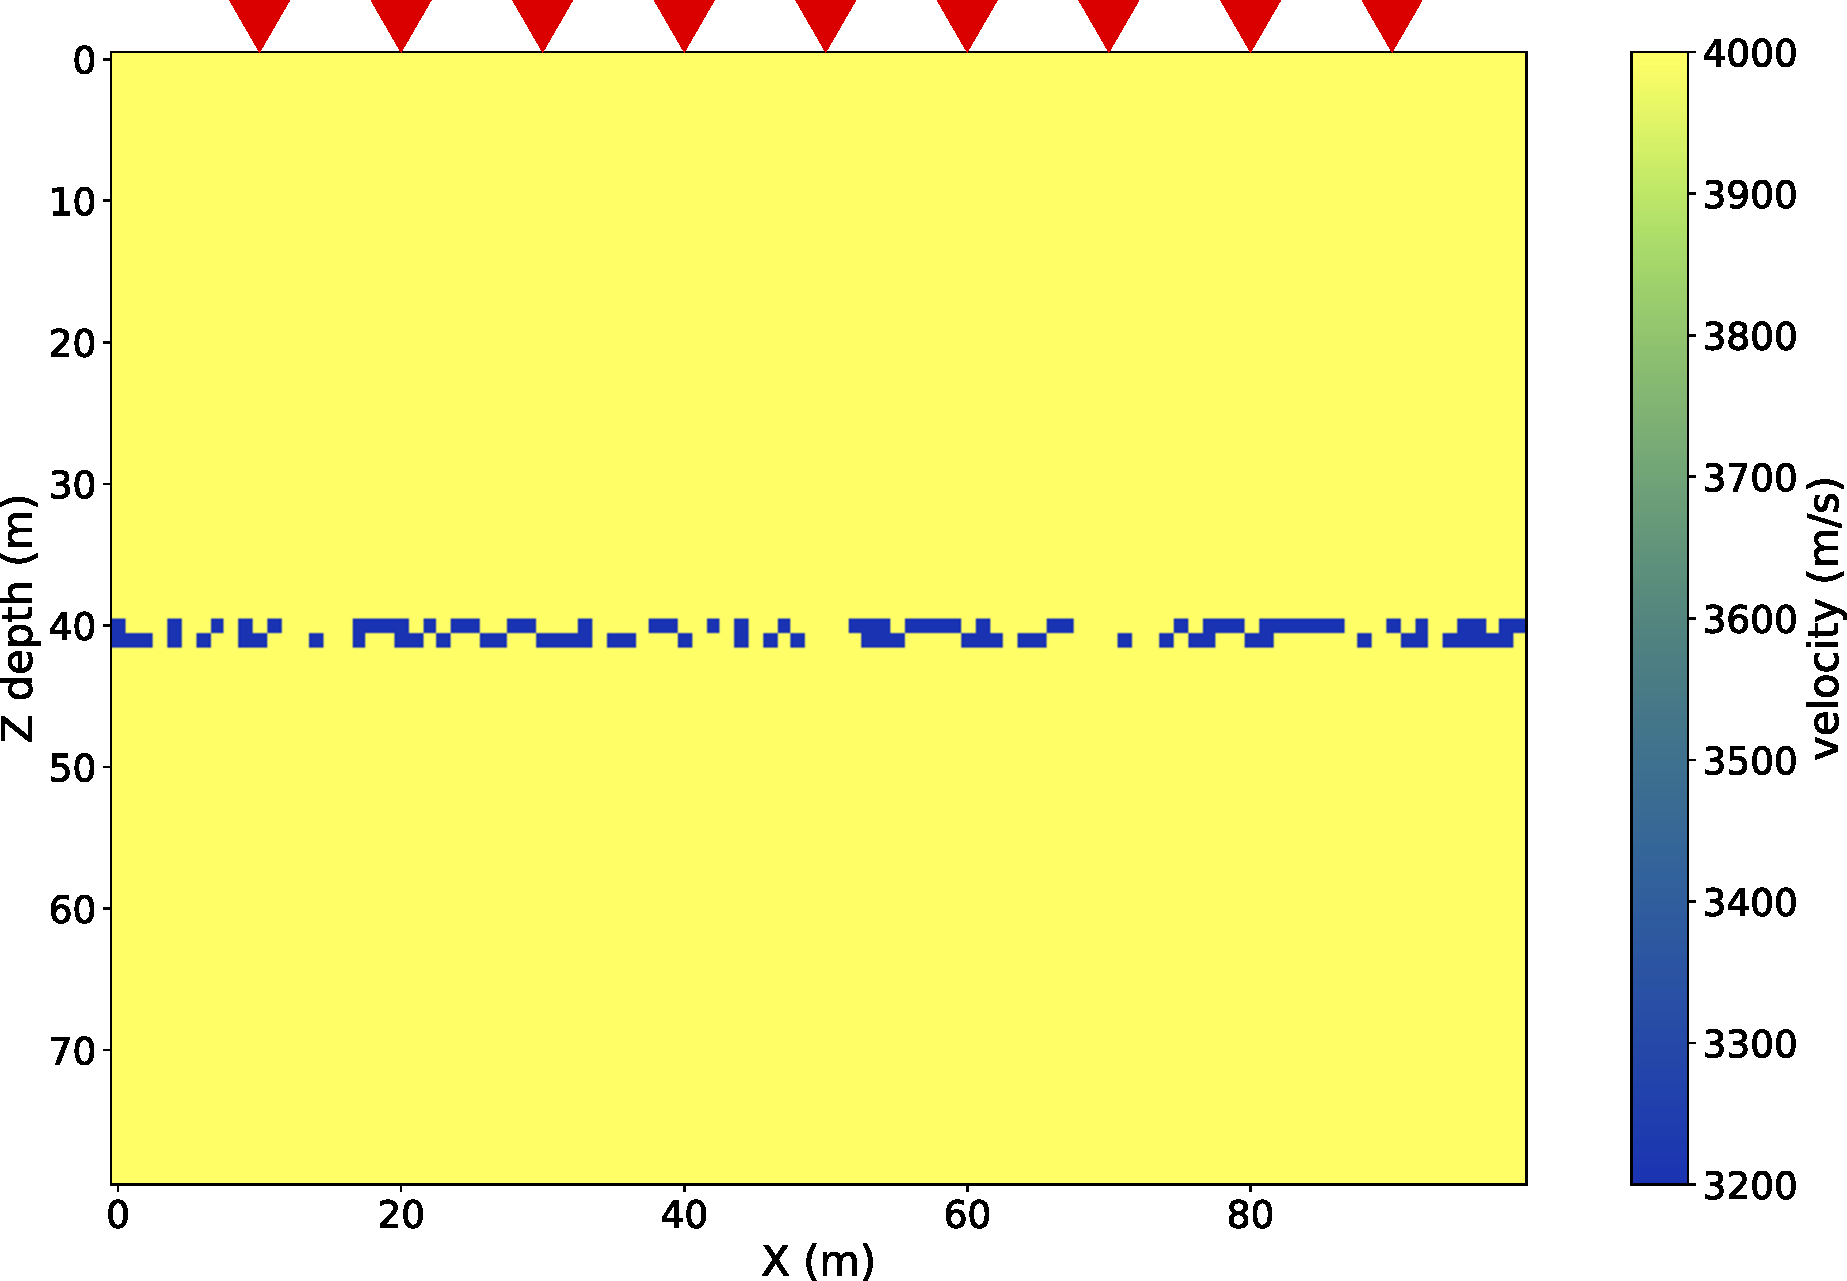
\includegraphics[height=4.5cm]{velocity_model}
				\caption[]{Velocity model with small irregular reflectors}
				\label{fig:vel_model}
			\end{figure}
		\end{column}
	
		\begin{column}{0.49\textwidth}
			\begin{figure}
				\centering
				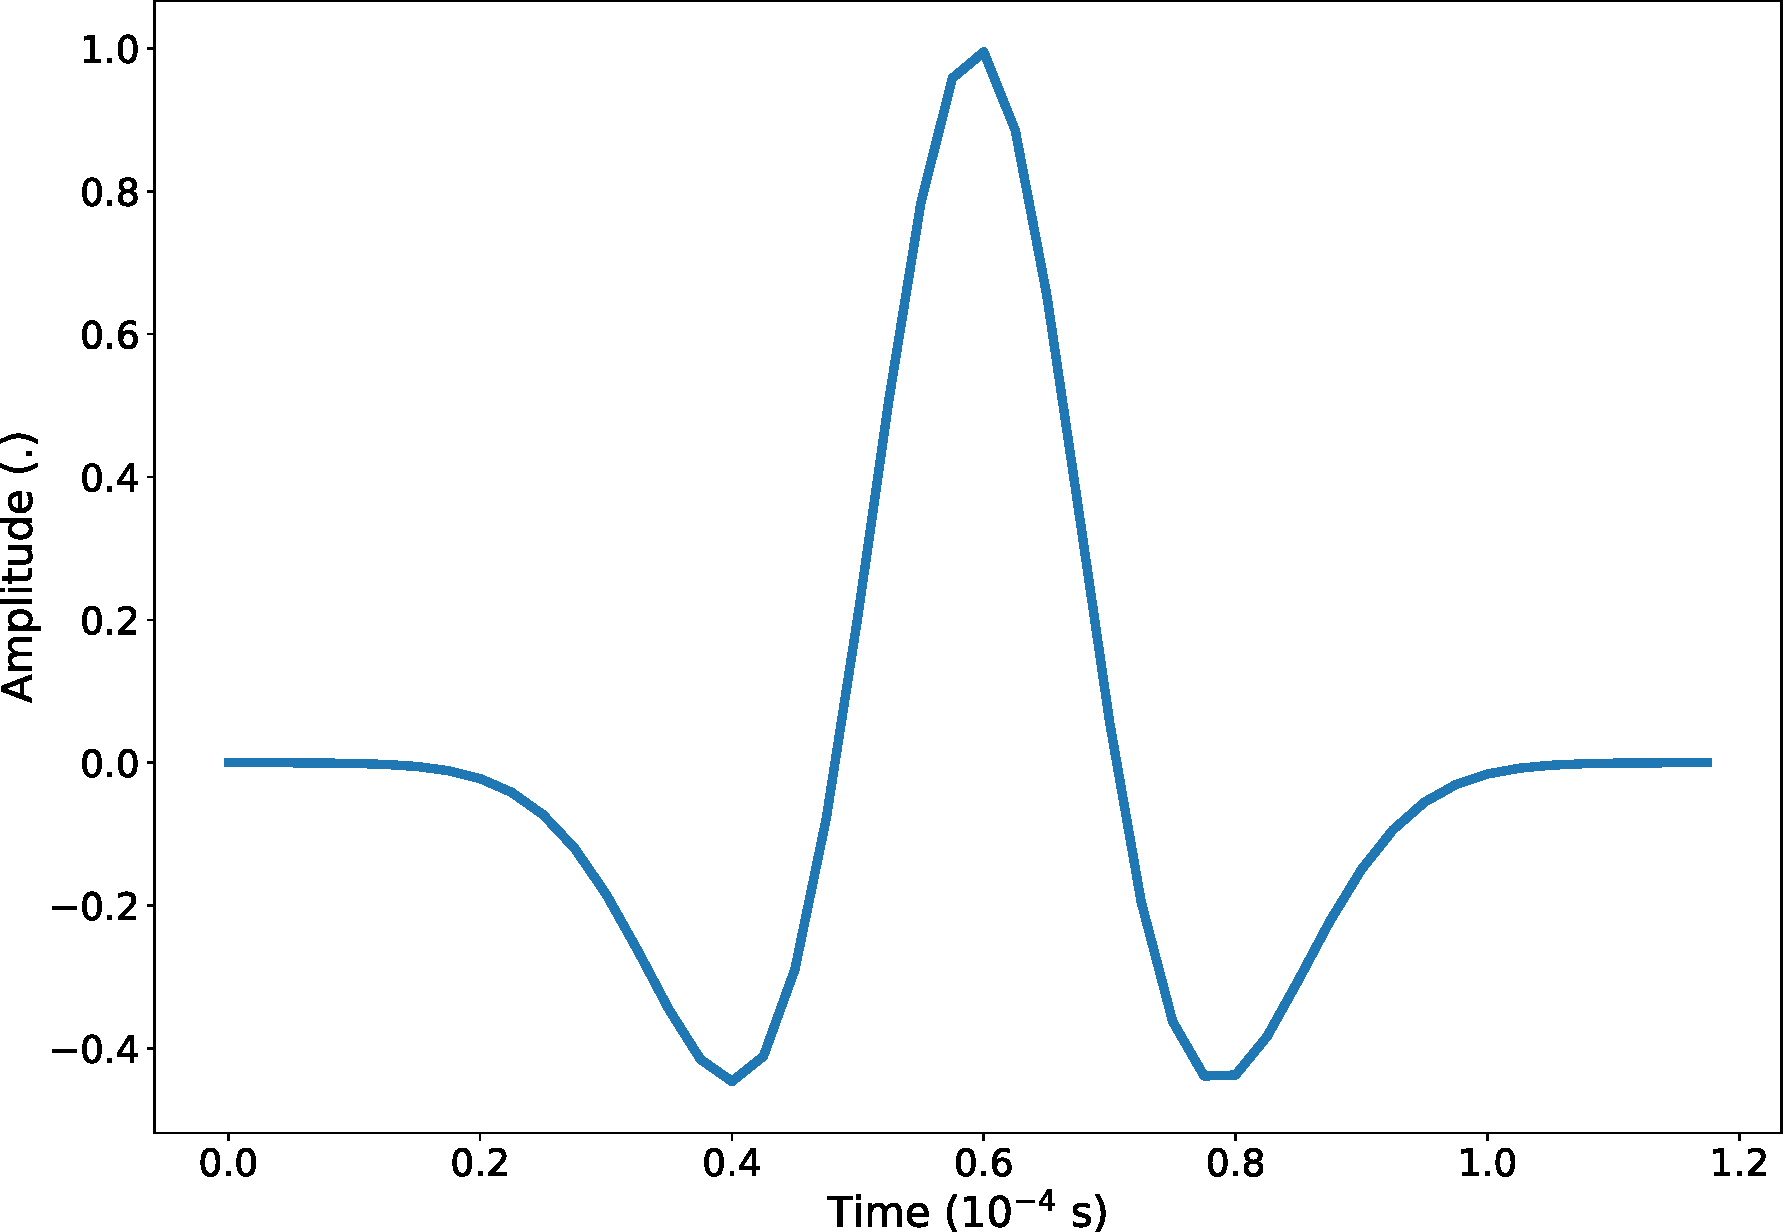
\includegraphics[height=4.5cm]{wavelet_ricker}
				\caption[]{Excitation source: ricker wavelet with $ f_c = 20\ kHz$}
				\label{fig:ricker}
			\end{figure}
		\end{column}
	\end{columns}
	
\end{frame}


\begin{frame}{Down-going \& up-going wavefields}
%	\centering
	\textit{Play .gif animations...}
\end{frame}


\begin{frame}{Shot-Gather: Pre-stack}
	\begin{figure}
		\centering
		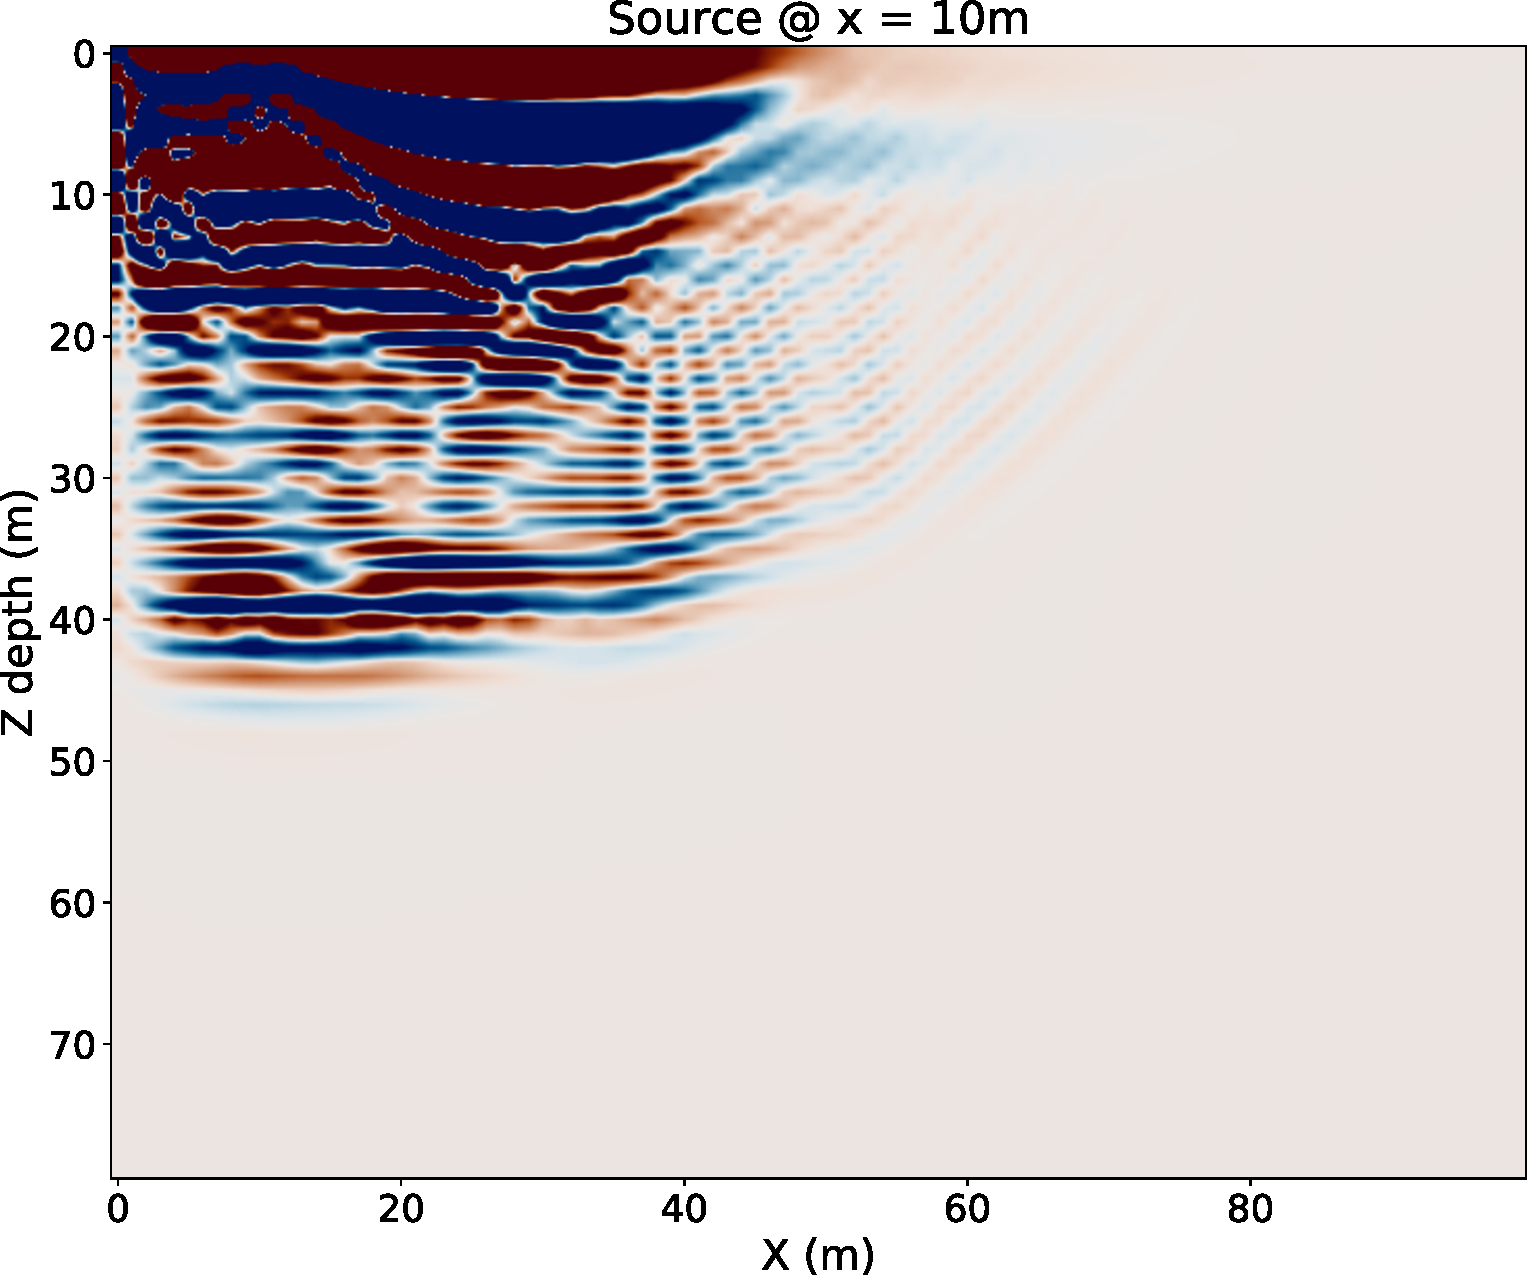
\includegraphics[height=3cm]{rtm_img_src=10m}
		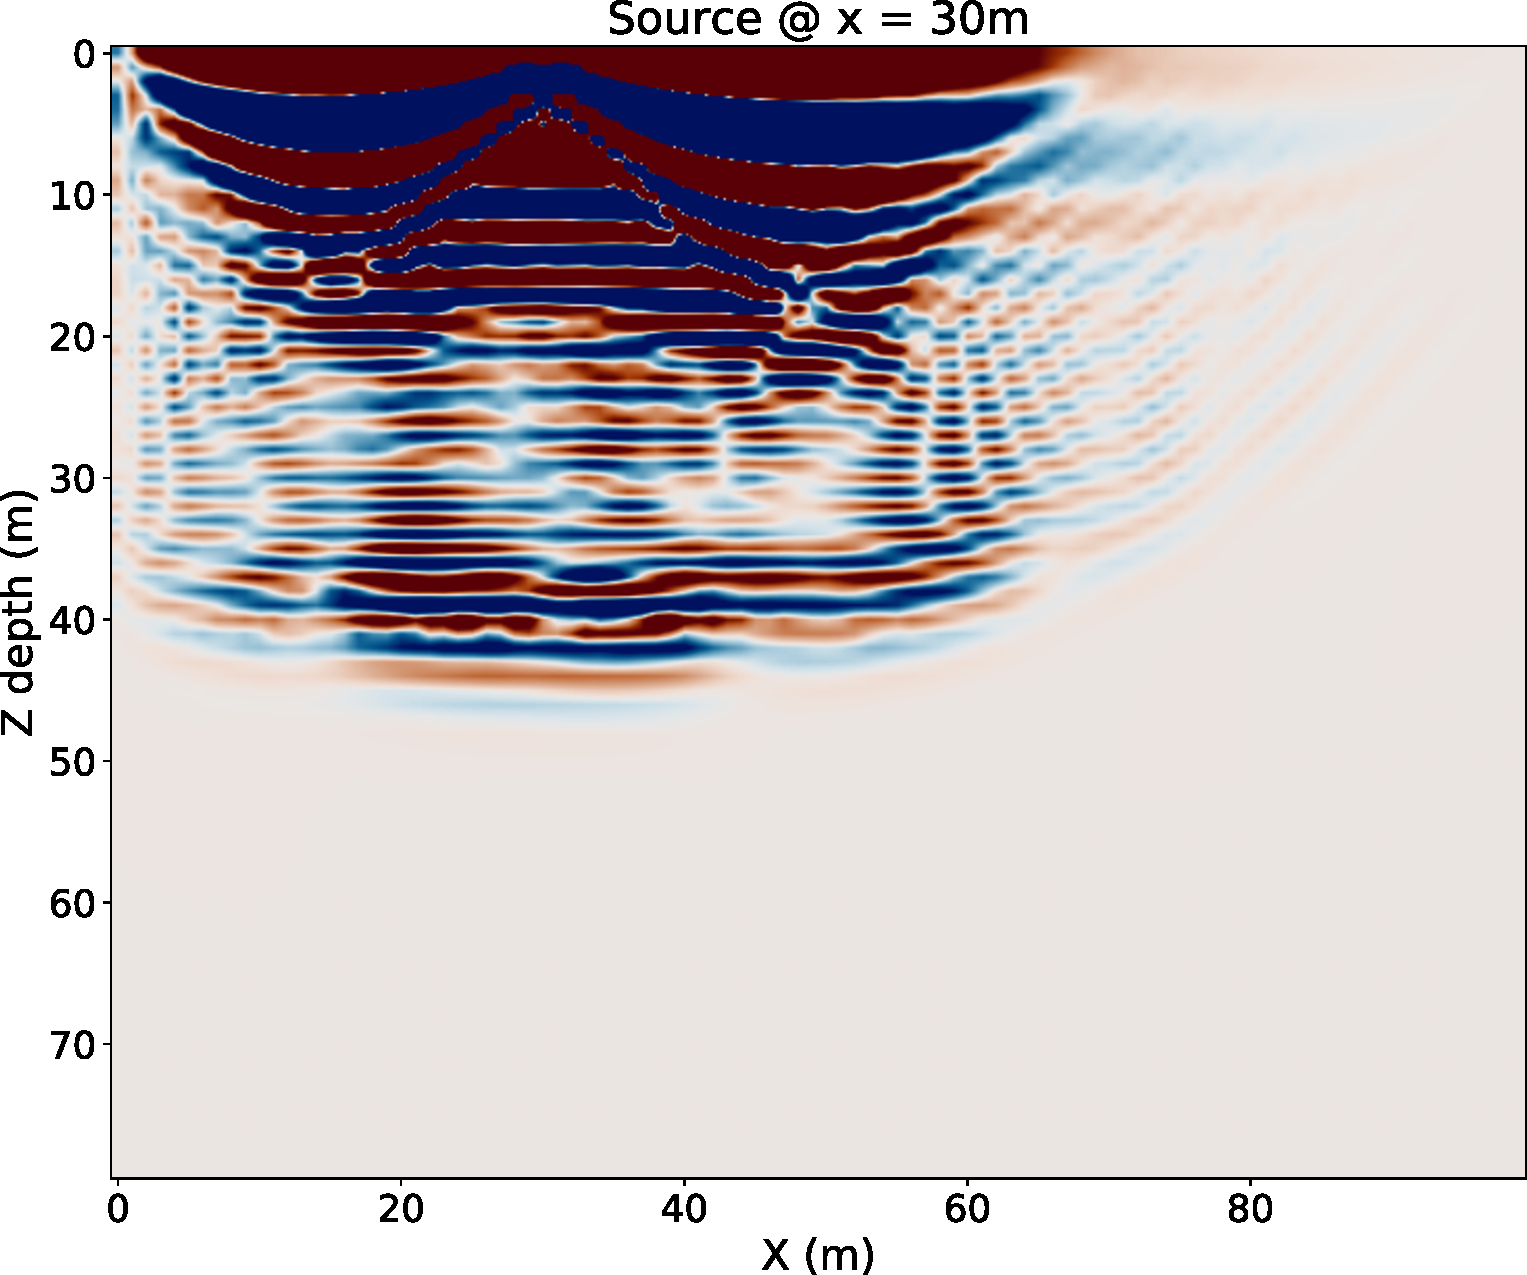
\includegraphics[height=3cm]{rtm_img_src=30m}
		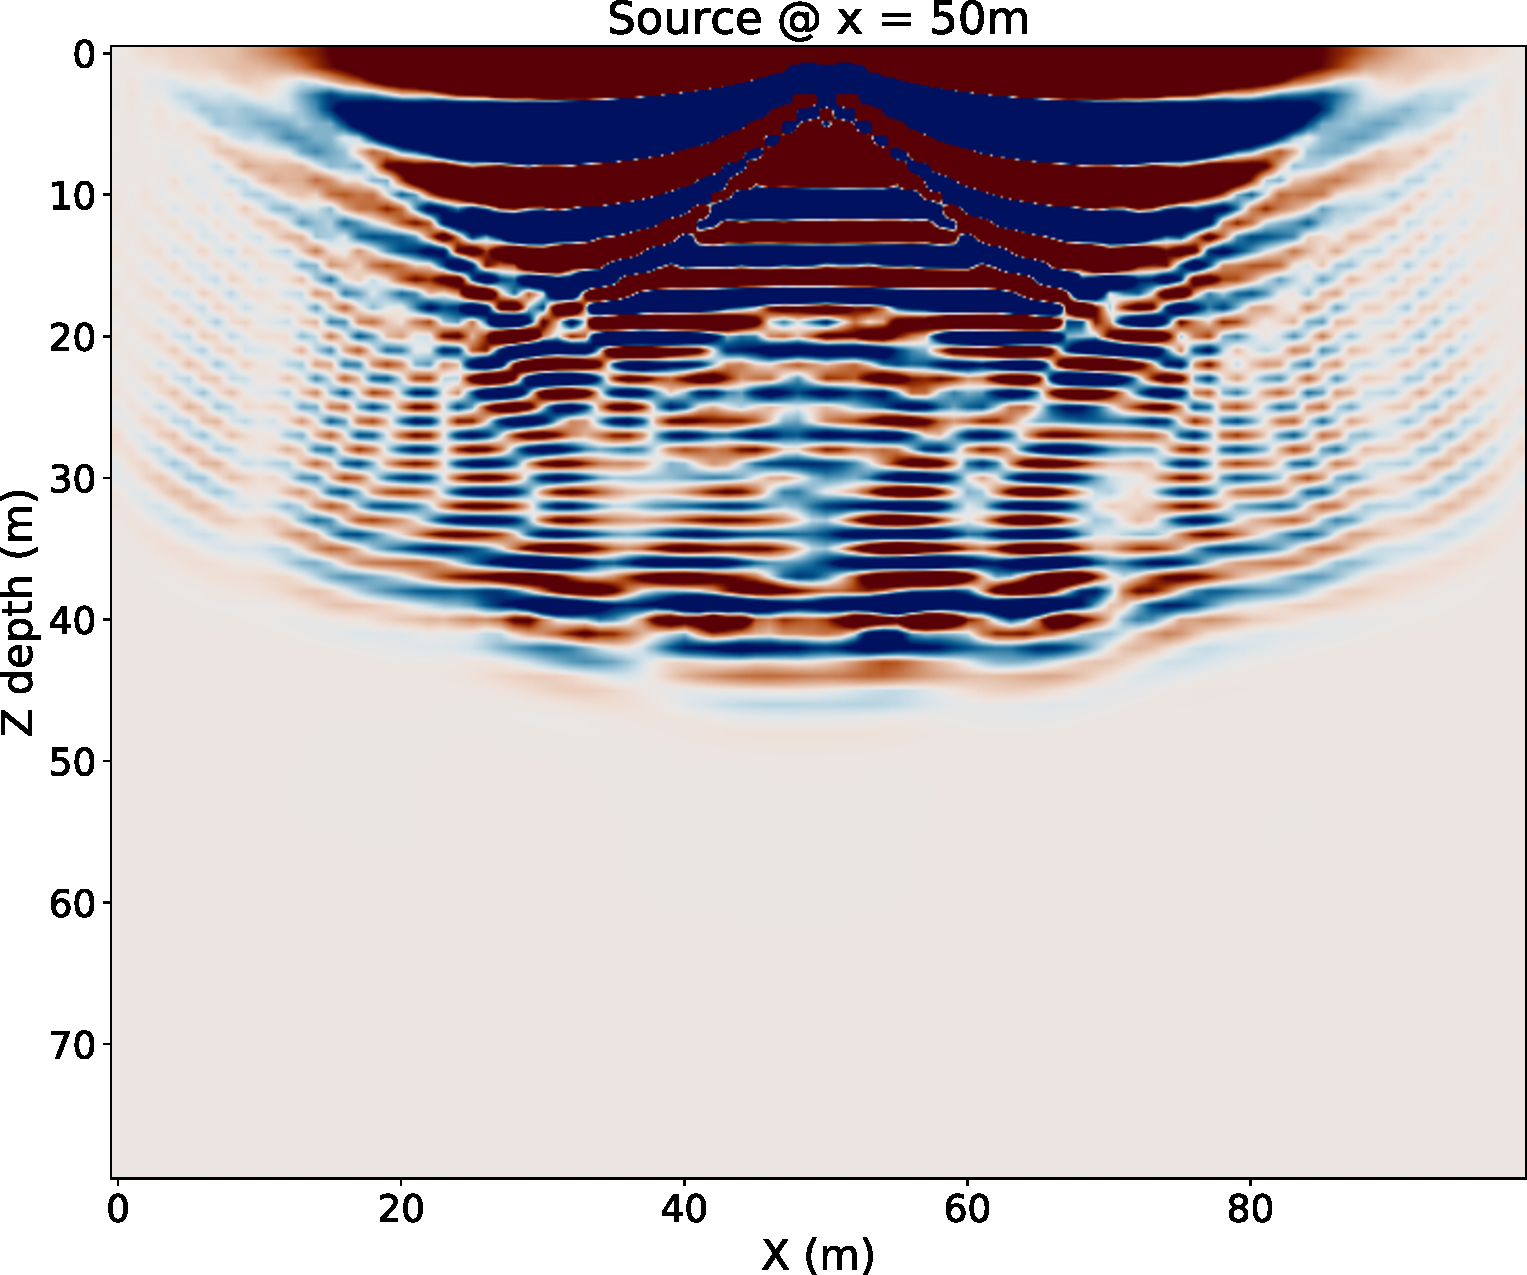
\includegraphics[height=3cm]{rtm_img_src=50m}
	\end{figure}
		
	\begin{figure}
		\centering
		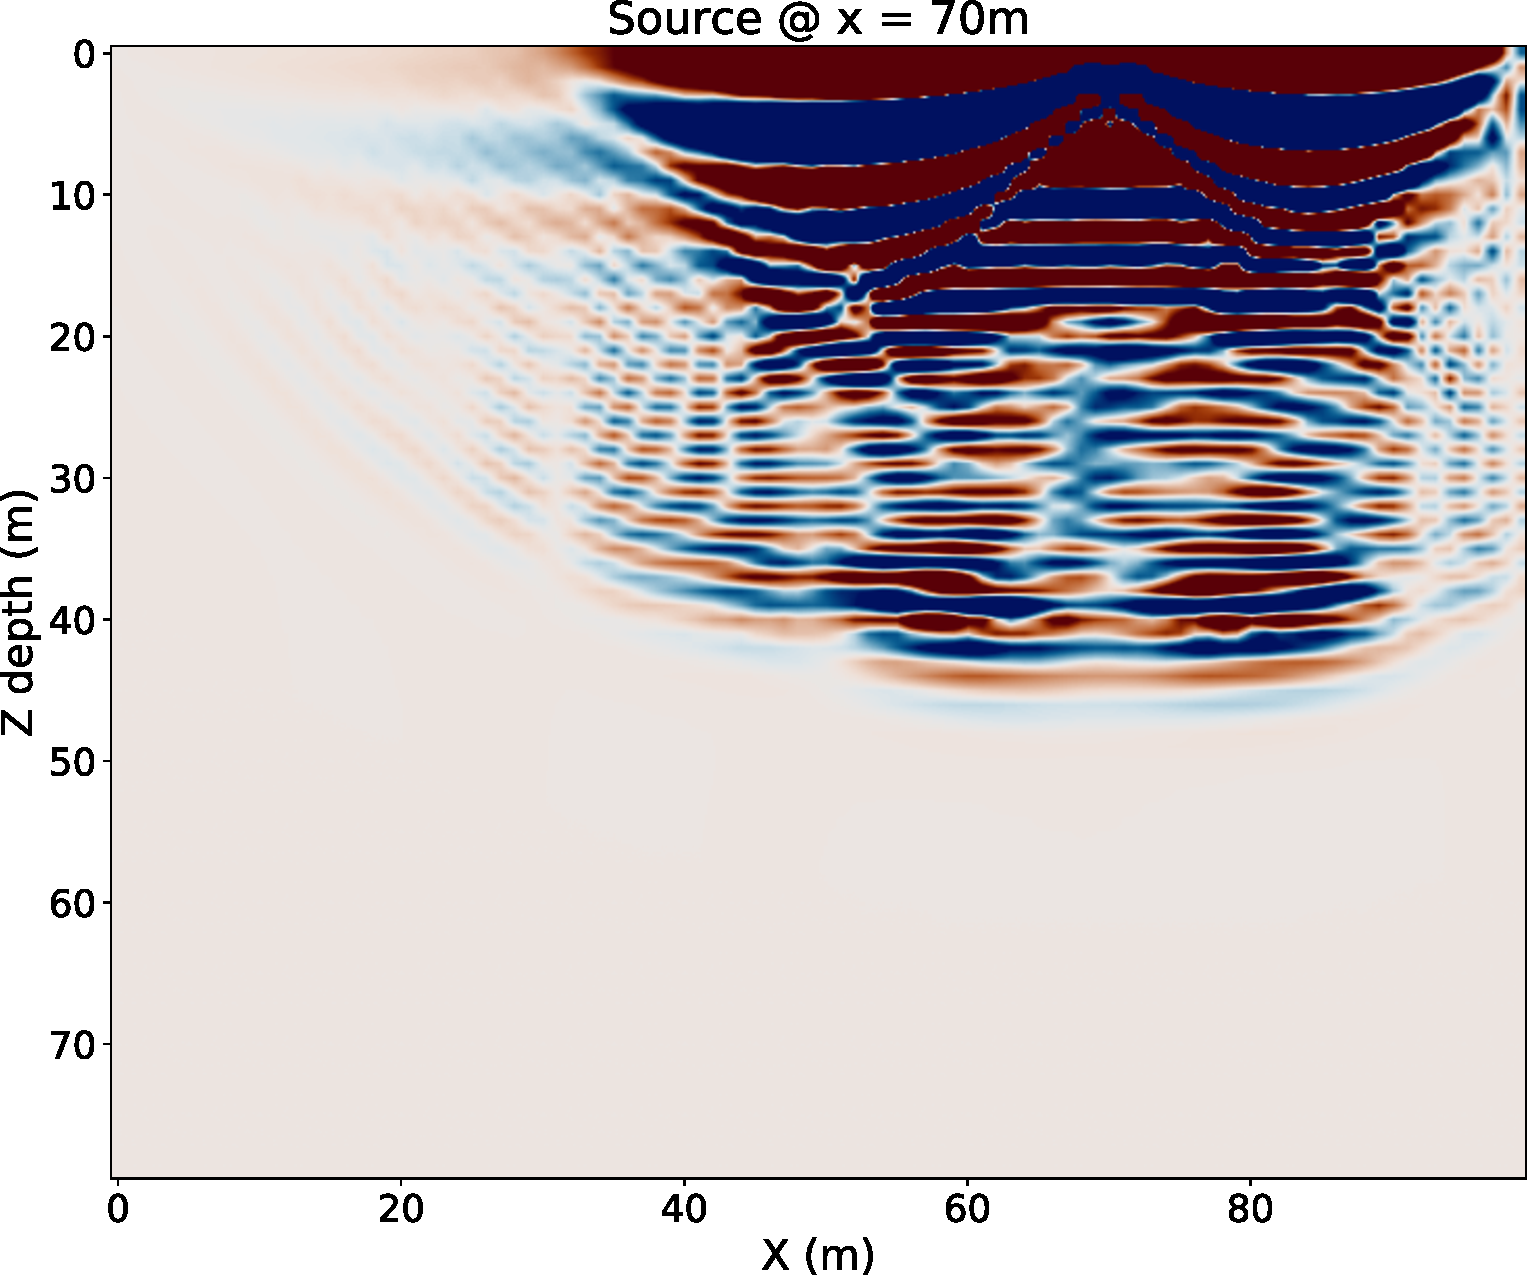
\includegraphics[height=3cm]{rtm_img_src=70m}
		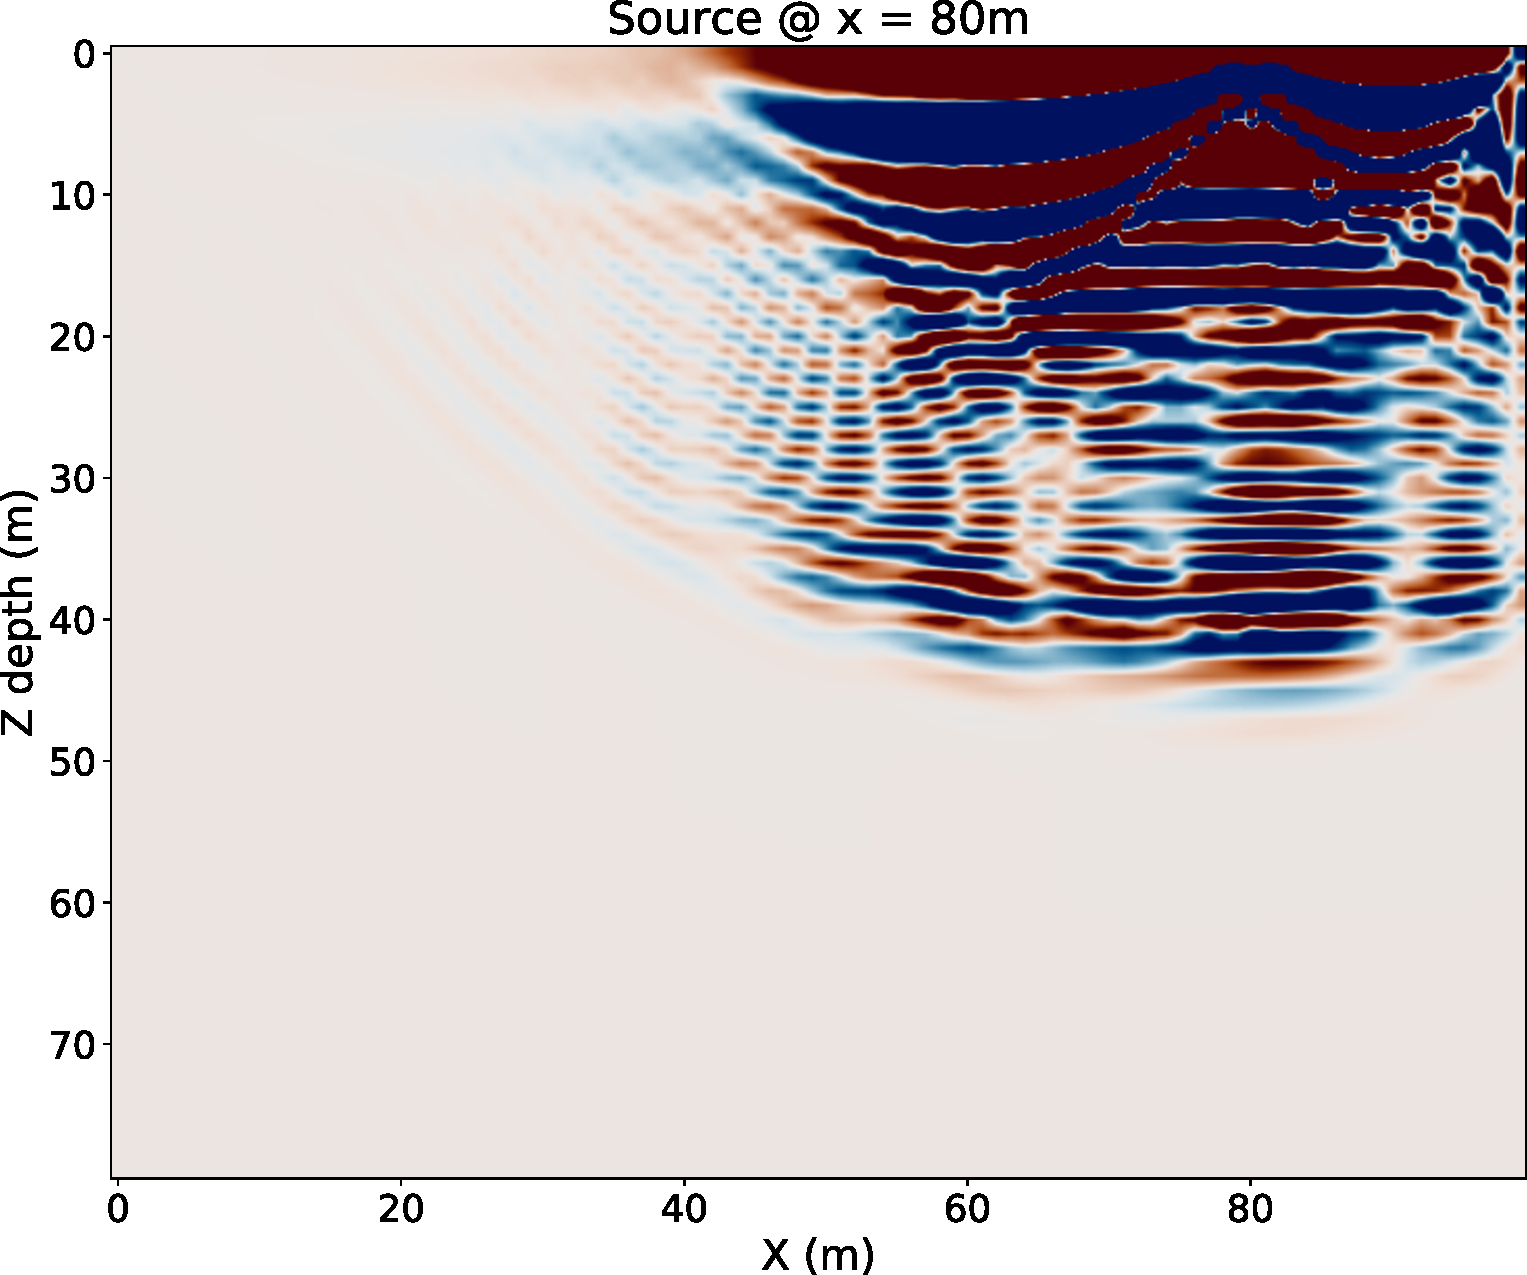
\includegraphics[height=3cm]{rtm_img_src=80m}
		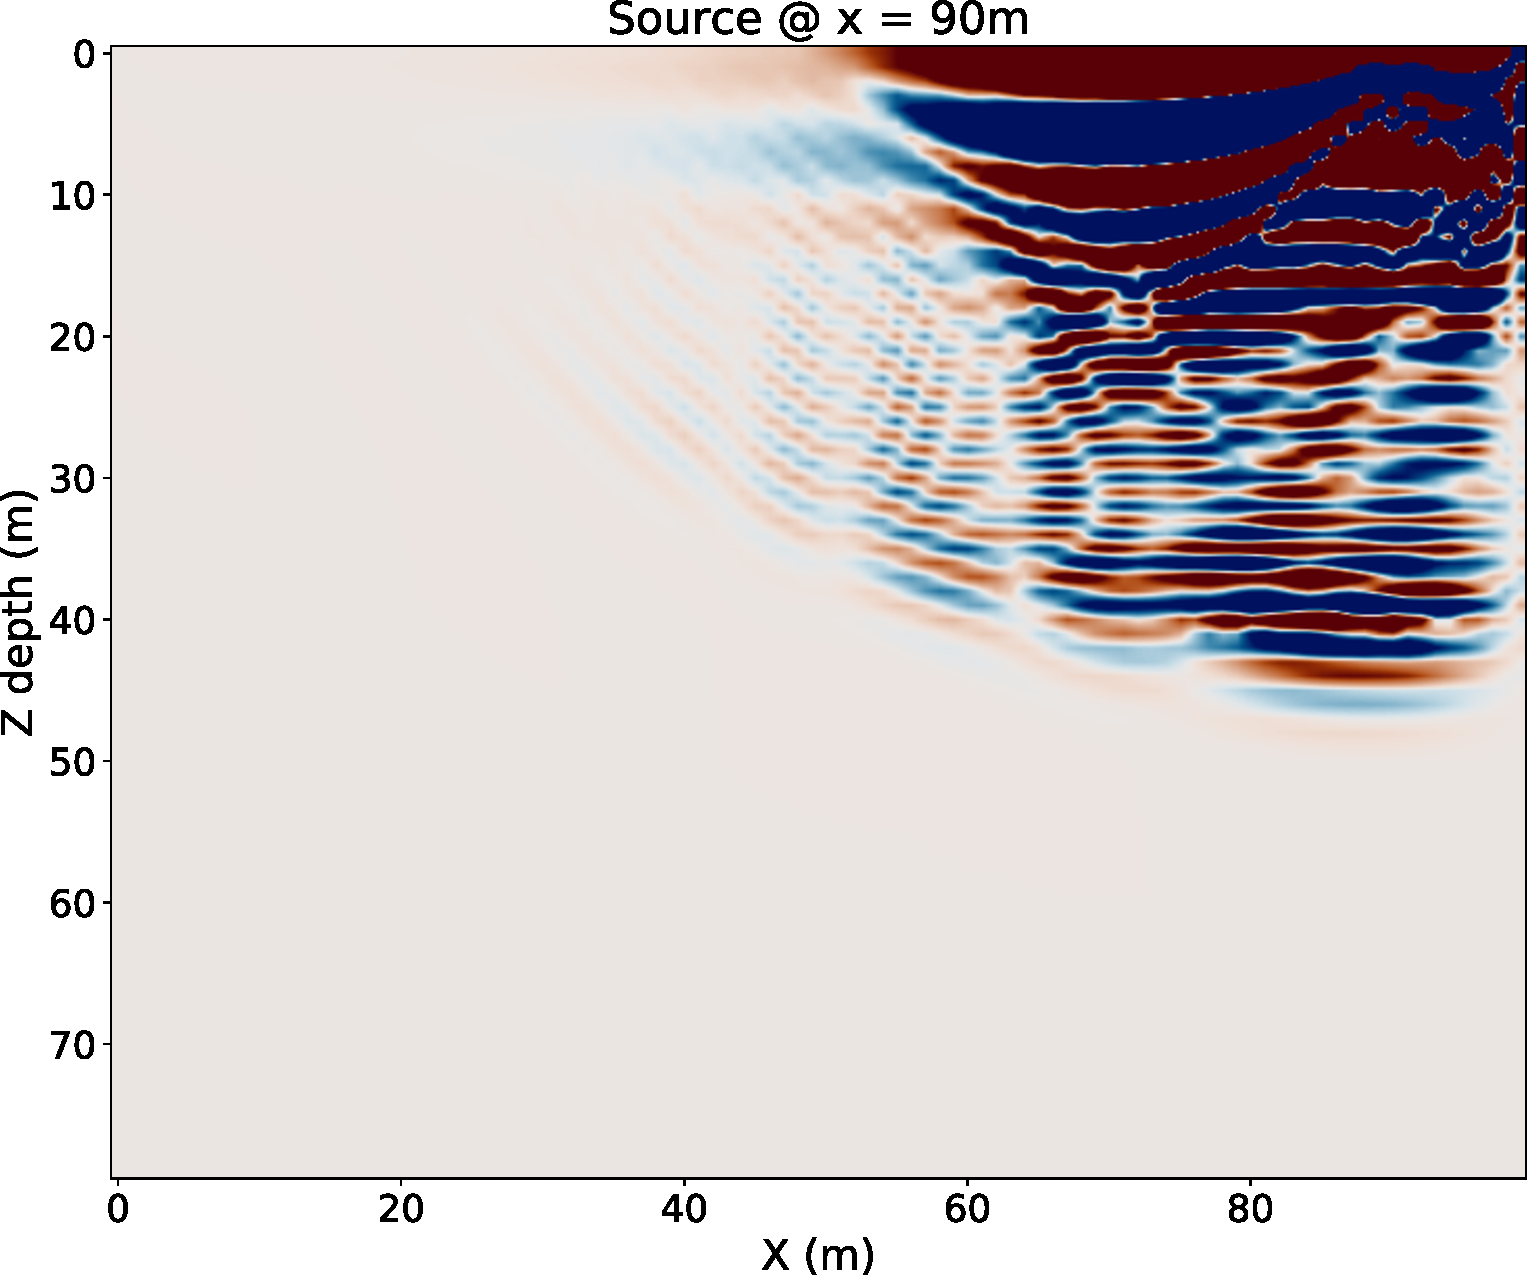
\includegraphics[height=3cm]{rtm_img_src=90m}
%		\caption[]{Velocity model with small irregular reflectors}
%		\label{fig:vel_model}
	\end{figure}

\end{frame}

\begin{frame}{Final Image}

	\begin{columns}
		\begin{column}{0.49\textwidth}
			\begin{figure}
				\centering
				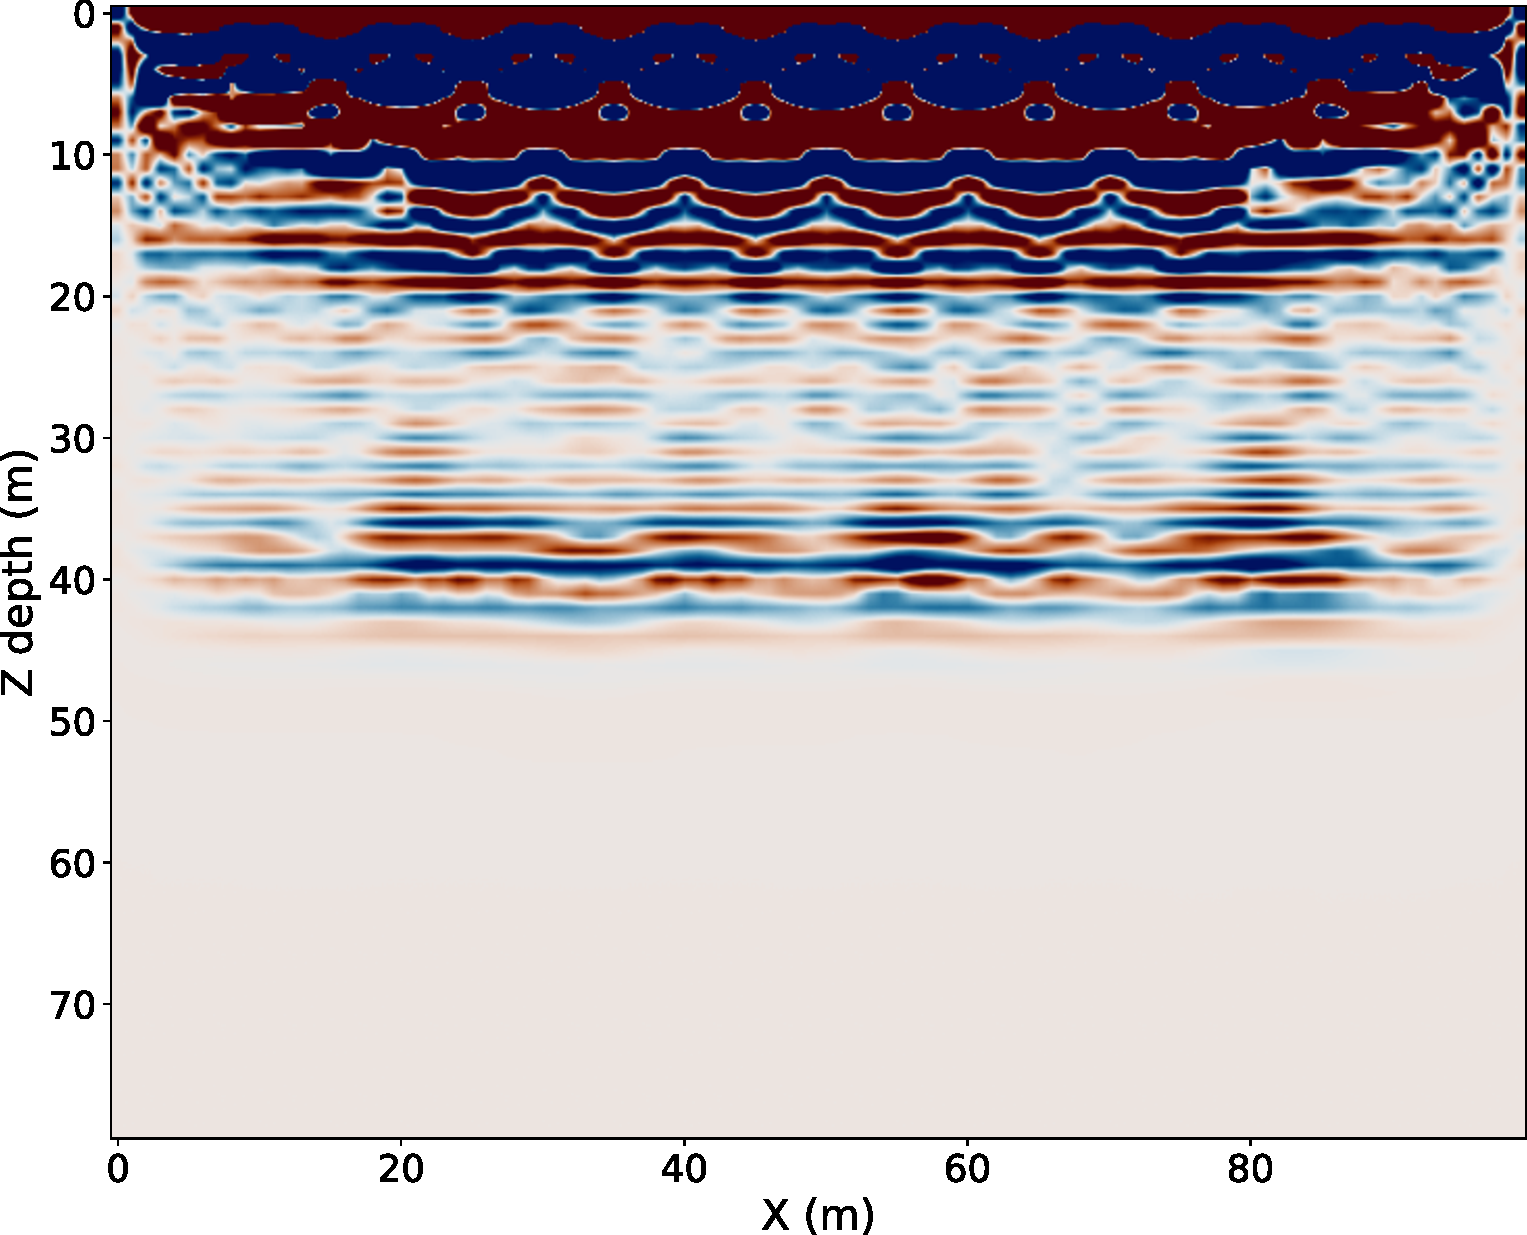
\includegraphics[height=5cm]{rtm_img_final}
				\caption[]{Stacked Image.}
				\label{fig:final}
			\end{figure}
		\end{column}
	
		\begin{column}{0.49\textwidth}
			\begin{figure}
				\centering
				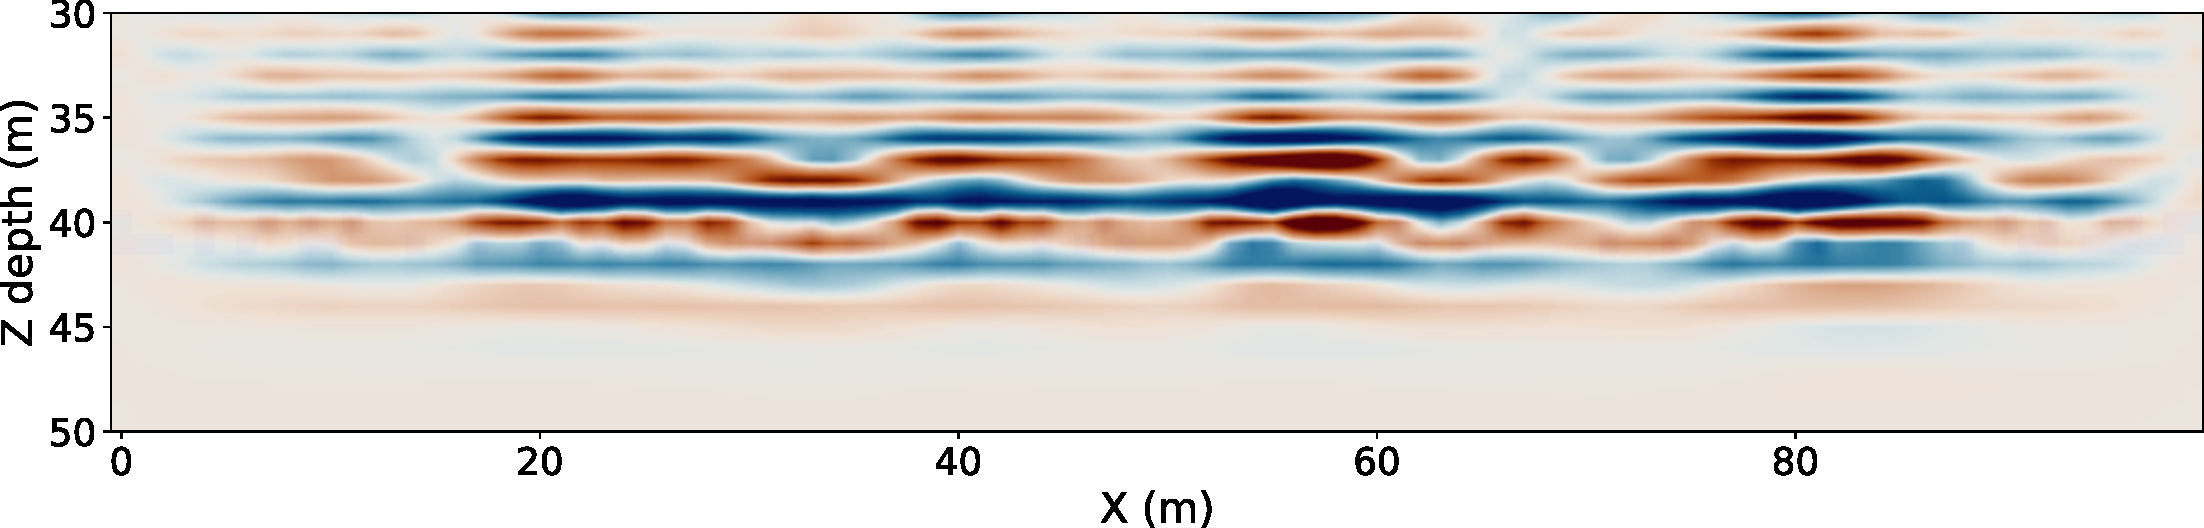
\includegraphics[width=7cm]{rtm_img_final_zoom}
				\caption[]{Final RTM image with overlayed velocity model.}
				\label{fig:final_zoom}
			\end{figure}
		\end{column}
	\end{columns}
	
\end{frame}


\end{document}
